Bộ nhớ (Memory) đóng vai trò là kho lưu trữ trung tâm cho cả lệnh chương trình 
và dữ liệu. 
Bộ nhớ sử dụng cổng dữ liệu lưỡng cực (Single bidirectional data port) có chức năng đọc và ghi, đảm bảo bộ nhớ không đọc và ghi cùng lúc.

\begin{figure}[H]
    \centering
    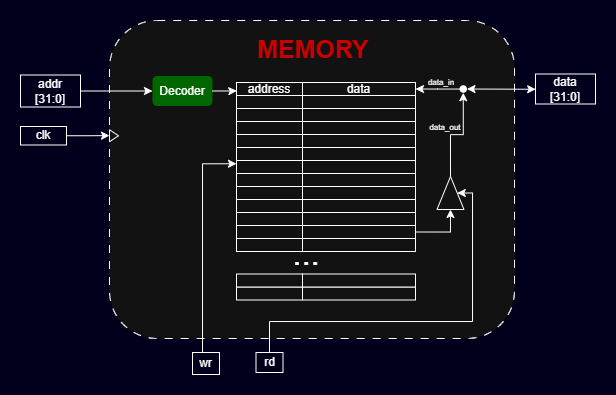
\includegraphics[width=0.9\textwidth]{Memory.png} 
    \caption{Sơ đồ khối Memory 32-bit}
    \label{fig:memory_internal}
\end{figure}

\textbf{Nguyên lý hoạt động:}
Khối Memory hoạt động đồng bộ với xung lên của clk và được quản lý bởi 
các tín hiệu điều khiển từ Controller. Thành phần của khối bao gồm:

\begin{itemize}
    \item \textbf{Giải mã địa chỉ (Address Decoding):} 
    Địa chỉ 32-bit từ ngõ vào sẽ đi qua khối Decoder. 
    giải mã vị trí hàng và cột trong mảng ô nhớ để chuẩn bị cho các thao tác truy xuất dữ liệu.
    
    \item \textbf{Ghi dữ liệu ($wr = 1$):} 
    Quá trình ghi diễn ra đồng bộ tại xung lên của clk. Khi tín hiệu \textit{wr} 
    được kích hoạt, dữ liệu từ cổng \textit{data} bên ngoài sẽ đi theo nhánh 
    \textit{data\_in} để đi vào ô nhớ đã được chọn bởi bộ giải mã.
    
    \item \textbf{Đọc dữ liệu và Trở kháng cao ($rd = 1$):} 
    Dữ liệu từ ô nhớ được đưa ra đường \textit{data\_out} 
    dẫn tới bộ đệm 3 trạng thái. 
    \begin{itemize}
        \item Khi $rd = 1$: Bộ đệm mở cho phép dữ liệu từ 
            \textit{data\_out} đi ra cổng giao tiếp bên ngoài.
        \item Khi $rd = 0$: 
        Bộ đệm sẽ đưa đầu ra về trạng thái trở kháng cao ($Z$), giúp "ngắt kết nối" bộ nhớ khỏi bus dữ liệu chung.
    \end{itemize}
\end{itemize}